\documentclass[11pt,a4paper]{article}
\usepackage[margin=2.0cm]{geometry}
\usepackage[T1]{fontenc}
\usepackage{amsmath}
\usepackage{graphicx}
\usepackage{booktabs}
\usepackage{tikz}
\usetikzlibrary{arrows.meta,positioning,fit,backgrounds}
\usepackage{caption}
\usepackage[compact]{titlesec}
\usepackage{xcolor}
\usepackage[hidelinks]{hyperref}
\captionsetup{font=small,labelfont=bf}
\setlength{\parskip}{2pt}
\setlength{\textfloatsep}{10pt plus 2pt minus 2pt}

\title{Timing Design and Controller Tuning\\for a CPSim-based Automotive Cyber-System\\[4pt]
\large Computer Modeling 2026 -- Final Project, Team 4}
\author{Youngbin Won\\{\small Dept.\ of Computer Science and Engineering, SNU}
\and Dogyu Lee\\{\small Dept.\ of Electrical and Computer Engineering, SNU}}
\date{November 2026}

\begin{document}
\maketitle

\begin{abstract}
We design the cyber-system of a simulated vehicle that is driven by two control software
components, lane keeping (LK) and cruise control (CC), together with four dummy components,
all mapped to a single ECU under rate-monotonic scheduling. For HW1 we choose task periods and
execution times that satisfy all utilization constraints while running the controllers as often
as possible, and we retune the controllers using data recorded from the real TORCS--CPSim setup.
The car completes a lap of E-Track 5 in \textbf{1:10.27} with one ECU and no deadline miss.
For HW2 we implement two loggers in the CPSim engine that record, in real-cyber-system time,
the data reads and writes of the control tasks and the release, start, finish, and deadline-miss
events of every job.
\end{abstract}

\section{Introduction}
Automotive control software runs as periodic tasks on ECUs, and the moment at which a task reads its
inputs and writes its outputs changes the behavior of the physical system it controls. CPSim
follows the approach of Functionally and Temporally Correct Simulation of Cyber-Systems for
Automotive Systems (RTSS 2017): the simulator first derives, for every job, the start and finish
times it would have on the real ECU, and then performs the job's data read and data write at those
times. The simulated control loop therefore experiences the same delays as the real one.

The final project has two parts. In HW1 we design the timing parameters of six software
components (SWCs) and modify the LK and CC code to make the car as fast as possible. In HW2 we
extend the CPSim engine with a read/write logger and a real-cyber-system schedule logger.

\section{System Overview}
Figure~\ref{fig:overview} shows the setup. TORCS runs on a Windows PC and simulates the vehicle and
the track. CPSim runs on an Ubuntu laptop connected by Ethernet. The CPSim GUI exports the system
design to \texttt{design.xml}, and the CPSim engine reads it, compiles the SWC code, and simulates the
ECU. Over a TCP connection, TORCS sends six sensor values (including speed, target speed, and the
lateral error of the car with respect to the lane), and the engine sends back the accelerator,
brake, and two steering commands after each control job.

The ECU runs six periodic SWCs: LK and CC, which have read and write constraints, and four dummy
components (SENSING, BRAKE, POWER, LOCAL), which only consume processor time. In the baseline
configuration all periods are 500\,ms, and the CC target speed is 40\,km/h.

\begin{figure}[t]
\centering
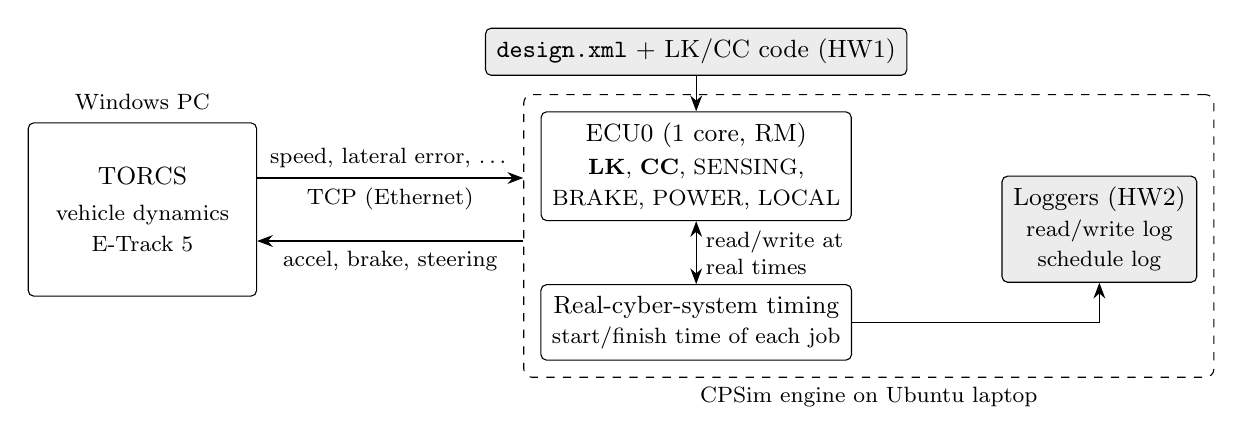
\begin{tikzpicture}[
  box/.style={draw,rounded corners=2pt,align=center,font=\small,inner sep=4pt},
  hw/.style={box,fill=gray!15},
  >={Stealth[length=2mm]}]
  % Windows PC
  \node[box,minimum width=2.9cm,minimum height=2.2cm] (torcs) {TORCS\\[2pt]{\footnotesize vehicle dynamics}\\{\footnotesize E-Track 5}};
  \node[font=\footnotesize,above=1pt of torcs] {Windows PC};
  % Engine internals
  \node[box,right=3.6cm of torcs,yshift=0.55cm,minimum width=3.2cm] (ecu)
       {ECU0 (1 core, RM)\\[1pt]{\footnotesize \textbf{LK}, \textbf{CC}, SENSING,}\\{\footnotesize BRAKE, POWER, LOCAL}};
  \node[box,below=0.8cm of ecu,minimum width=3.2cm] (rcs)
       {Real-cyber-system timing\\{\footnotesize start/finish time of each job}};
  \node[hw,right=1.9cm of ecu,yshift=-0.8cm,minimum width=2.3cm] (logs)
       {Loggers (HW2)\\{\footnotesize read/write log}\\{\footnotesize schedule log}};
  \node[hw,above=0.45cm of ecu,minimum width=3.2cm] (design)
       {\texttt{design.xml} + LK/CC code (HW1)};
  \begin{scope}[on background layer]
    \node[draw,dashed,rounded corners=3pt,fit=(ecu)(rcs)(logs),inner sep=6pt,label={[font=\footnotesize]below:CPSim engine on Ubuntu laptop}] (engine) {};
  \end{scope}
  \draw[->] (design) -- (ecu);
  \draw[<->] (ecu) -- node[right,font=\footnotesize,align=left]{read/write at\\real times} (rcs);
  \draw[->] (rcs.east) -| (logs.south);
  \draw[->] ([yshift=0.4cm]torcs.east) -- node[above,font=\footnotesize]{speed, lateral error, \dots}
            node[below,font=\footnotesize]{TCP (Ethernet)} ([yshift=0.4cm]torcs.east -| engine.west);
  \draw[<-] ([yshift=-0.4cm]torcs.east) -- node[below,font=\footnotesize]{accel, brake, steering}
            ([yshift=-0.4cm]torcs.east -| engine.west);
\end{tikzpicture}
\caption{System overview. Shaded boxes mark the parts changed in HW1 (design and controller code)
and HW2 (loggers).}
\label{fig:overview}
\end{figure}

\section{HW1: Timing Design}
\subsection{Constraints}
Each SWC has a period $T$ and an execution time $C$ (BCET $=$ WCET $= C$, deadline $= T$).
The rules are $20 \le T \le 500$, $C \ge 20$, both multiples of 10, and a minimum utilization
$U = C/T$ that depends on the period: 0.1 for $T \in (250,500]$, 0.2 for $T \in (100,250]$, and 0.5 for
$T \le 100$. Any deadline miss gives a zero grade, and each ECU beyond the first costs one point.
We therefore use a single ECU.

\subsection{Design space}
The controllers react faster when their periods are shorter, so the goal is to minimize the LK
and CC periods subject to schedulability. The four dummies need at least
$4 \times 0.1 = 0.4$ of the processor, which they get at $T = 500$, $C = 50$.
The minimum utilization jumps from 0.2 to 0.5 at $T = 100$, which matters most for the design.
With $T_{LK} = 100$, LK alone needs $U = 0.5$. Together with the dummies this leaves exactly 0.1 for CC,
which forces $T_{CC} = 500$ and a total utilization of exactly 1.0. That design is schedulable
because the periods are harmonic, but it has no slack at all, and CC would run only every 500\,ms.
Any $T_{LK} < 100$ exceeds a utilization of 1. Above 100\,ms, the smallest legal period is 110\,ms
with $C = 30$ ($C = 20$ gives $U = 0.18 < 0.2$). We enumerated all legal parameter combinations and
checked each with exact response-time analysis. Running both LK and CC at 110\,ms is the fastest
schedulable design that keeps a safety margin.

\subsection{Selected design}
Table~\ref{tab:design} lists the final parameters and the worst-case response times under RM.
Ties between equal periods are broken by task order, so CC runs before LK. The total utilization is
$2 \cdot 30/110 + 4 \cdot 50/500 = 0.945$, and every job finishes at least 50\,ms before its
deadline. The hyper period is $\mathrm{lcm}(110, 500) = 5500$\,ms.

\begin{table}[t]
\centering\small
\caption{Final timing design on one ECU (RM, phase 0). $R$ is the worst-case response time.}
\label{tab:design}
\begin{tabular}{lrrrrrc}
\toprule
SWC & Period $T$ & Exec.\ $C$ & $U$ & $R$ & Slack & Read/Write \\
\midrule
CC      & 110 & 30 & 0.273 &  30 &  80 & Y \\
LK      & 110 & 30 & 0.273 &  60 &  50 & Y \\
SENSING & 500 & 50 & 0.100 & 110 & 390 & N \\
BRAKE   & 500 & 50 & 0.100 & 220 & 280 & N \\
POWER   & 500 & 50 & 0.100 & 330 & 170 & N \\
LOCAL   & 500 & 50 & 0.100 & 440 &  60 & N \\
\midrule
Total   &     &    & 0.945 &     &     &   \\
\bottomrule
\end{tabular}
\end{table}

Each dummy SWC is mapped to its own source file and not to the LK or CC code.

\section{HW1: Controller Design}
\subsection{Lane keeping}
The original LK is a proportional controller: the steering command equals the lateral error,
clamped to $\pm 10000$. With a 110\,ms update interval, this controller and our first variant
(which added a large derivative term) both made the car weave. To tune the controller
systematically, we recorded the signals exchanged between TORCS and CPSim by capturing the TCP
traffic on the Ethernet link during test runs.

From the recorded data we identified a discrete model of the lateral motion with one step per LK
job. Let $L_k$ be the lateral error, $\Delta L_k = L_k - L_{k-1}$, and $u_k$ the steering command.
A least-squares fit gives
\begin{equation}
\Delta L_k = 0.39\,\Delta L_{k-1} + 0.05\,\Delta L_{k-2} - 0.32\,u_{k-1} + 0.01\,u_{k-2} + 0.10\,u_{k-3} + d_k ,
\end{equation}
where $d_k$ collects the effect of the track curvature. The fit has $R^2 = 0.83$ on one run and
$0.84$ on another. In closed-loop simulation the model reproduces the observed problem: the
previous controller is predicted to reverse the steering direction about 2.8 times per second.
We then searched proportional, derivative, and integral gains on this model, and also tested them
with the steering response scaled up to twice its value, since the car reacts more strongly at
higher speed. The selected controller is
\begin{equation}
u_k = 0.7\,L_k + 0.3\,(L_k - L_{k-1}) + \mathrm{sat}_{\pm 3000}\Big(0.01 \sum_{i \le k} L_i\Big),
\qquad |u_k| \le 10000 ,
\end{equation}
where the saturated integral term removes the steady offset in long corners without wind-up.

Table~\ref{tab:lk} compares the two controllers on the same 130\,s portion of two real runs, and
Figure~\ref{fig:steer} shows a 15\,s excerpt. The tuned controller reverses the steering ten times
less often, never saturates, and keeps the car four times closer to the lane center, even though the car
drives 25\% faster.

\begin{table}[t]
\centering\small
\caption{Lane keeping before and after tuning, measured on real runs (5--135\,s of each run).}
\label{tab:lk}
\begin{tabular}{lrr}
\toprule
 & Previous (P + strong D) & Tuned PID \\
\midrule
Mean speed (km/h)                    & 79.2 & 101.4 \\
Steering direction changes per second & 3.98 & 0.39 \\
Time at steering limit               & 27.2\% & 0.0\% \\
Mean $|u|$                           & 6004 & 553 \\
RMS lateral error                    & 3762 & 836 \\
Max.\ $|$lateral error$|$            & 9840 & 3557 \\
\bottomrule
\end{tabular}
\end{table}

\begin{figure}[t]
\centering
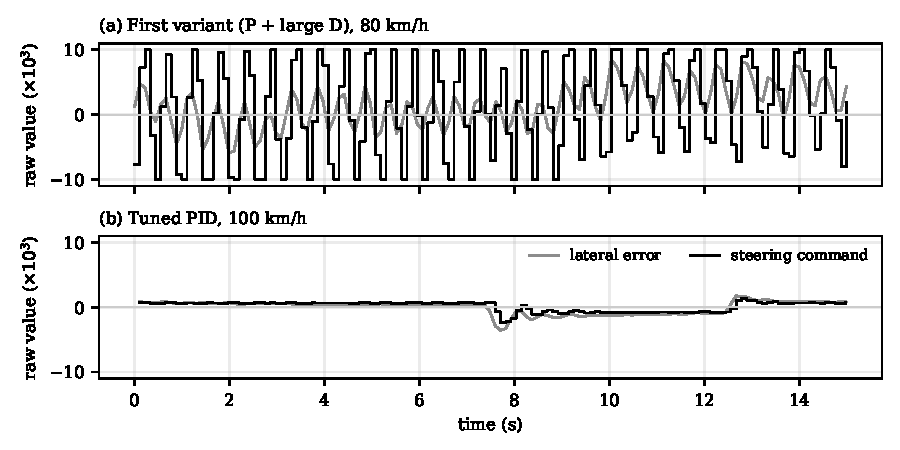
\includegraphics[width=0.82\linewidth]{figures/steering.pdf}
\caption{Lateral error and steering command on the real setup. (a) Previous controller: the
steering switches between the limits every few jobs. (b) Tuned PID controller at a higher speed.}
\label{fig:steer}
\end{figure}

\subsection{Cruise control}
CC computes its target from the TARGET\_SPEED signal and an offset. TORCS reports speed in units of
$10^{-4}$\,km/h, and with the offset of the provided code the target is about 80\,km/h. We raised the
target to 100\,km/h. The original on/off logic is kept: CC requests acceleration below the target and
releases the throttle above it. As a safety measure, CC also reads the lateral error and releases the
throttle when $|L| > 15000$. At that point the steering limit of LK can no longer correct the
deviation. Acceleration resumes when $|L| < 8000$. The hysteresis prevents rapid switching.
During the final run the lateral error never reached this threshold while driving, so this rule
did not affect the lap time.

\subsection{Handling stale sensor data}
In two test runs, TORCS kept sending packets at the normal rate, but their contents stayed exactly the
same for 1.5\,s and 3\,s while the car kept moving. Because the values were captured on the network
link, the freeze originated on the TORCS side. We did not identify its cause. During the first
occurrence, LK kept applying its last steering command and the car left the track. A moving car never
reports exactly the same lateral error or speed twice in a row 110\,ms apart. We therefore treat an
input that is unchanged for two consecutive jobs as stale: LK then steers straight and resets its
state, and CC releases the throttle. In the second occurrence the car slowed from about 83 to 64\,km/h
and continued normally once fresh data arrived.

\section{HW1: Results}
Figure~\ref{fig:lap} shows the TORCS screen after the final run. The best lap time is
\textbf{1:10.27}, which is 89.7\,s faster than the 2:40 baseline time and therefore reaches the
maximum score of 10 points. Only one ECU is used. The engine log of this run covers 74 hyper periods
(407\,s of simulated time). All 10\,656 jobs were released, started, and finished, with no deadline
miss.

\begin{figure}[t]
\centering
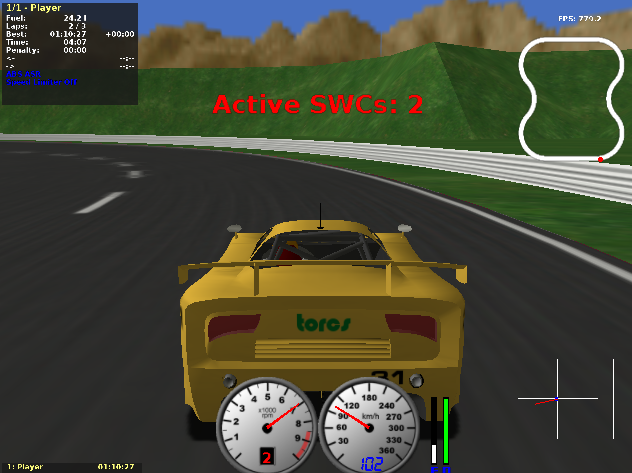
\includegraphics[width=0.48\linewidth]{Team4_HW1_lap_time.png}
\caption{TORCS after the final run on E-Track 5: best lap time 1:10.27.}
\label{fig:lap}
\end{figure}

\section{HW2: Logger Implementation}
\subsection{Read/write logger}
For a task with a read or write constraint, the engine executes each job's function in the
simulator when the wall-clock time reaches the job's start time on the real ECU. We log a READ entry with the job's
real start time before the function runs, and a WRITE entry with its real finish time after it
returns (\texttt{Job::run\_function}). One entry is written for each data item: ACCEL\_VALUE,
TARGET\_SPEED, SPEED, and CC\_TRIGGER (read) and BRAKE and ACCEL (write) for CC; \texttt{rtU.read1}
and \texttt{rtU.read2} (read) and \texttt{rtY.write3} and \texttt{rtY.write4} (write) for LK. The
simulator executes jobs in a different order and at different times than the real ECU, so the
entries of one hyper period are buffered, sorted by real time, and written at the end of the hyper
period. Jobs that never run on the real ECU (no real start time) produce no entries. The logged
tasks are selected with \texttt{log\_task} in \texttt{settings.txt}, which accepts a comma-separated
list such as \texttt{"LK, CC"}.

\subsection{Real-cyber-system schedule logger}
At the beginning of each hyper period, after the engine has computed the real-cyber-system timing
of all jobs, we generate one event per job for release, start, and finish, plus a DEADLINE MISS
event at the deadline if the job did not start, did not finish, or finished late. Events are sorted
by time. At equal times, releases come first, then finishes, then starts, then misses, so a job that
finishes exactly at its deadline is not a miss. Job identifiers in the engine restart every hyper
period, so we number jobs from the start of the simulation, $j = (r - \phi)/T + 1$ for release time $r$
and phase $\phi$. Each job is printed as J\textit{<task><job>}, e.g., J12 is the second job of task 1.
Events that fall after the end of the current hyper period are kept and written with the next one.
Listing~\ref{lst:logs} shows the beginning of both logs from the final run.

\begin{figure}[h]
\centering
\begin{minipage}[t]{0.52\linewidth}\scriptsize
\begin{verbatim}
[ TIME ] [ READ/WRITE ] [ TASK NAME ] [ DATA NAME ]
0     READ    CC    ACCEL_VALUE
0     READ    CC    TARGET_SPEED
0     READ    CC    SPEED
0     READ    CC    CC_TRIGGER
30    WRITE   CC    BRAKE
30    WRITE   CC    ACCEL
30    READ    LK    rtU.read1
30    READ    LK    rtU.read2
60    WRITE   LK    rtY.write3
60    WRITE   LK    rtY.write4
\end{verbatim}
\end{minipage}\hfill
\begin{minipage}[t]{0.40\linewidth}\scriptsize
\begin{verbatim}
[ TIME ] [ JOB ID ] [ EVENT TYPE ]
0        J11        RELEASED
0        J21        RELEASED
...
0        J11        STARTED
30       J11        FINISHED
30       J21        STARTED
60       J21        FINISHED
60       J31        STARTED
110      J12        RELEASED
\end{verbatim}
\end{minipage}
\captionof{figure}{Beginning of \texttt{Team4\_read\_write.log} (left) and
\texttt{Team4\_schedule.log} (right) from the final run (columns compressed). Task 1 is CC,
task 2 is LK, and task 3 is SENSING.}
\label{lst:logs}
\end{figure}

\subsection{Engine fixes and verification}
While implementing the loggers we fixed three problems in the engine and the project setup:
\texttt{log\_task} was parsed only up to the first space, so \texttt{"LK, CC"} dropped CC; entries with
time $-1$ from jobs that never ran on the real ECU appeared in the log; and the engine extracts
the SWC code starting from the first line that contains the file name, so renamed copies such
as \texttt{Team4\_CC.cpp} failed to compile until the name was added in a comment at the top.
We tested the loggers in a local sandbox with a stub TORCS server. The tests covered the baseline
design, our final design, and an overloaded design. In the overloaded design, the expected DEADLINE MISS
events appear, and the missed jobs produce no read/write entries. We also checked the loggers on the
real setup.

\section{Conclusion}
With a single ECU, the controllers can run every 110\,ms, which is the fastest rate that both satisfies the
utilization rules and leaves a safety margin. Most of the improvement in lap time came from the
controller design. A model identified from real driving data showed that the steering problem
was caused by the gains, not by the sampling rate. After retuning the gains and raising the cruise target, the car
completed a lap in 1:10.27 without any deadline miss. The two loggers report the data accesses and
the job schedule in real-cyber-system time and form a basis for checking the timing of future designs.

\end{document}
